\documentclass[a4paper]{report}

\usepackage[utf8]{inputenc} %Accent
%\usepackage{libertine} %Font
\usepackage[english, francais]{babel} %langue

\usepackage{graphicx} %Include fig
\usepackage{caption} %center the caption
\usepackage{subfig} %Include subfig
\usepackage{lastpage} %ref LastPage 
\usepackage{fancyhdr} % headers,footers
\usepackage{multicol} % minipages
\usepackage{textcomp} 
\usepackage{lscape}   %Format paysage
\usepackage{fancybox} %Image arrière plan
\usepackage{amsmath} %\mathbb, \mathit...
\usepackage{amssymb} 
\usepackage{color} %couleurs
\usepackage{float}
\usepackage[hidelinks]{hyperref} %Liens intradoc et url
\usepackage{titlepic}

%\usepackage{algorithm}
%\usepackage{algorithmic} %Algo en pseudo code
%\usepackage{algorithm2e} %for psuedo code

%\usepackage{boxedminipage} %Surligner

%\newcounter{apppage} % Annexes

%Dossier contenant les figures
\graphicspath{{figures/}}

%Mise en page
\voffset -1.5 cm
\textheight 24.3 cm
\topmargin 0 cm
\headheight 0 cm
%\headsep 0.6 cm
\textwidth 16.5 cm
\evensidemargin 0 cm
\marginparsep 0 cm
\marginparwidth 0 cm
\oddsidemargin -.5 cm

%Titre
\title{Pattern recognition\\Report\\Assignment n°1}
\author{Audrey Brouard \and Antoine Honoré}



%Type de numérotation des sections & sous-sections
\renewcommand{\thesection}{\Roman{section}}
\renewcommand{\thesubsection}{\thesection.\arabic{subsection}}

%\renewcommand\thesubfigure{(\alph{subfigure})}
\setlength{\parindent}{0cm}
\setlength{\parskip}{1ex plus 0.5ex minus 0.2ex}
\newcommand{\hsp}{\hspace{20pt}}
\newcommand{\HRule}{\rule{\linewidth}{0.5mm}}

%email
\newcommand{\email}[1]{\href{mailto:#1}{\color{blue} \textsf{#1}}}

%Bibliography
\bibliographystyle{apalike}

%Environnement insersion image
\newcommand{\img}[3]{\begin{figure}[!h] \centering \includegraphics[scale=#2]{#1}\captionsetup{justification=centering} \caption{#3} \label{#1} \end{figure}}
  % commande \img{nom image}{scale}{legende}

%TODO
\newcommand{\todo}[1]{{ \Large \textbf{ \colorbox{yellow}{\color{blue} TODO:}}~#1}}

%pushright
\newenvironment{pushright}[1]{\textbf{#1}
\begin{itemize}\item[\hspace{12pt}]}{\end{itemize}
}

%%%%%%%%%%%%%%%%%%%%%%%%%%%%%%%%%%%%%%%%%%%%%%%%%%%%%%%%%%%%%%
%%%%%%%%%%%%%%%%%%%%%%%%%%%%%%%%%%%%%%%%%%%%%%%%%%%%%%%%%%%%%%
%%%%%%%%%%%%%%%%%%%%%%%%%%%%%%%%%%%%%%%%%%%%%%%%%%%%%%%%%%%%%%
\pagestyle{fancy}  % Activation en-tête et pied de page

%En-tête
\fancyhead[L]{Audrey Brouard \& Antoine Honoré - Pattern recognition - Assignment n°1}
%\fancyhead[C]{}
%\fancyhead[R]{}
% Pied de page
\newcommand{\width}{3cm}
%\fancyfoot[L]{ \includegraphics[width=\width]{logo-gipsa} }
\fancyfoot[C]{ \thepage~/~\pageref{LastPage} }
%\fancyfoot[R]{ \includegraphics[width=\width]{logo-phelma} }

\titlepic{
\includegraphics[scale=0.6]{kth-logo}}

\begin{document}

%%%%%%%%%%%%%%%% TITLE %%%%%%%%%%%%%%%%
\begin{titlepage}
  \begin{sffamily}
    \begin{center}

      \textsc{ }\\[1.5cm]

      % % Title
      % \vspace{3cm}
      \HRule \\[0.4cm]
      { \Huge \bfseries Pattern recognition system\\Exercise Project\\[0.4cm] }
      \HRule \\[2.5cm]
      \textsc{\LARGE Report Assignment n°2}~\\[2.5cm]
% Authors
      \begin{minipage}{0.4\textwidth}
        \begin{flushleft} \large
          \emph{\textbf{Student}}\\
          Antoine \textsc{Honoré}\\
          \email{honore@kth.se}
          ~\\~\\~\\
        \end{flushleft}
      \end{minipage}
      \hfill
      \begin{minipage}{0.4\textwidth}
        \begin{flushright} \large
          \emph{\textbf{Student}}\\
          Audrey \textsc{Brouard}\\
          \email{brouard@kth.se}
        \end{flushright}
      \end{minipage}
      % 
\includegraphics[scale=0.5]{kth-logo}

     

      \vfill

      % Bottom of the page
      {\large 2015 Period 1}

    \end{center}
  \end{sffamily}

\end{titlepage}


%%% Local Variables:
%%% TeX-master: "master"
%%% End:
%%%%%%%%%%%%%%%%%%%%%%%%%%%%%%%%%%%%%%%%%%%%%%%%%%%%%%%%%%%%%%%%
%%%%%%%%%%%%%%%%%%%%%%%%%%%%%%%%%%%%%%%%%%%%%%%%%%%%%%%%%%%%%%%%
%%%%%%%%%%%%%%%%%%%%%%%%%%%%%%%%%%%%%%%%%%%%%%%%%%%%%%%%%%%%%%%%
%%%%%%%%%%%%%%%%%%%%%%%%%%%%%%%%%%%%%%%%%%%%%%%%%%%%%%%%%%%%%%%%
%%%%%%%%%%%%%%%%%%%%%%%%%%%%%%%%%%%%%%%%%%%%%%%%%%%%%%%%%%%%%%%%
\section{}

Let us calculate $P(S_{t}=j)$ $ \forall j\in\{1,2\} $ and for t = 1,2,3,...

We will do it for t = 1 and t = 2, and notice that the probabilities are constant $\forall t$.

\begin{itemize}
  \item For t = 1, the probabilities are given by the matrix $q_{j}$. Thus, $P(S_{1}=1) = 0.75$ and $P(S_{1}=2) = 0.25$.\\
\end{itemize}
$\forall t\geq 2$, we will use the following formula :

	\begin{itemize}
	  \item $P(S_{t}=j) = \sum_{i=1}^{2} P({S_t}=j,S_{t-1}=i) = \sum_{i=1}^{2} P(S_t=j|S_{t-1}=i)P(S_{t-1}=i)$\\
	\end{itemize}

For the case t = 2, we have :
\begin{itemize}
  \item $P(S_t=j) = \sum_{i=1}^{2} a_{ij} q_i$
\end{itemize}

We thus obtain $P(S_{2}=1)=0.75$  and $P(S_{2}=2)=0.25$.
We immediately notice that \[\forall i~P(S_{2}=i) = P(S_{1}=i)\]
By recurrency, we have $\forall t~\Pr(S_{t}=j)$ constant.

\section{}
After we generated 10 000 state integers, we found the following probabilities :
\[\Pr(S_{t} = 1) = 0.7525~and~\Pr(S_{t} = 2) = 0.2475\]

\section{@HMM/rand}
\subsection{Theorical calculation}
Let us now calculate $E[X_{t}]$ and $Var[X_{t}]$.

\begin{itemize}
	\item 
	$E[X_{t}]$ : the book gives the formula $E[X]=E_{S}[E_{X}[X|S]]$, and according to the two different possible values of S, X density probability function is either $b_{1}$ or $b_{2}$.
	
	Then, for j = 1, $E[X|S]=\mu_{1}$ ;
	and for j = 2, $E[X|S]=\mu_{2}$.
	
	
	$E[X]=P(S=1)*\mu_{1} + P(S=2)*\mu_{2} = 0 + 3*0.25 = 0.75$.
	
\end{itemize}

\begin{itemize}
	\item $Var[X_{t}]$ : according to the book, $Var[X_{t}]=E_{S}[Var_{X}[X|S]] + Var_{S}[E_{X}[X|S]]]$.
	
	Thanks to the same observation as before, the expression becomes :
	
	$Var[X_{t}]=E_{S}[Var_{X}[X|S]] + E_{S}[(E_{X}[X|S])^2] - E_{S}[E_{X}[X|S] ]^2$
	
	$Var[X_{t}]=[0.75 * \sigma_{1}^2 + 0.25*\sigma_{2}^2] + [0.75*\mu_{1}^2+0.25*\mu_{2}^2] - 0.75^2 = 1.75+0.25*9-0.75^2=3.4375$.
\end{itemize}
\pagebreak
\subsection{Measures}
One point on a graph represent the mean (figure \ref{hmmrand:mean}) and the variance (figure  \ref{hmmrand:var}) of T=10000 scalar output. There is 20 points on each graph.  This shows that the experimental values are close from the theoretical ones

As we can see on the figures  the experimental values are close from the theoretical ones.
\begin{figure}[!h]
\centering
    \subfloat[Variance of 10000 samples computed 20 times $E(Var(X)) \simeq 2.919$]{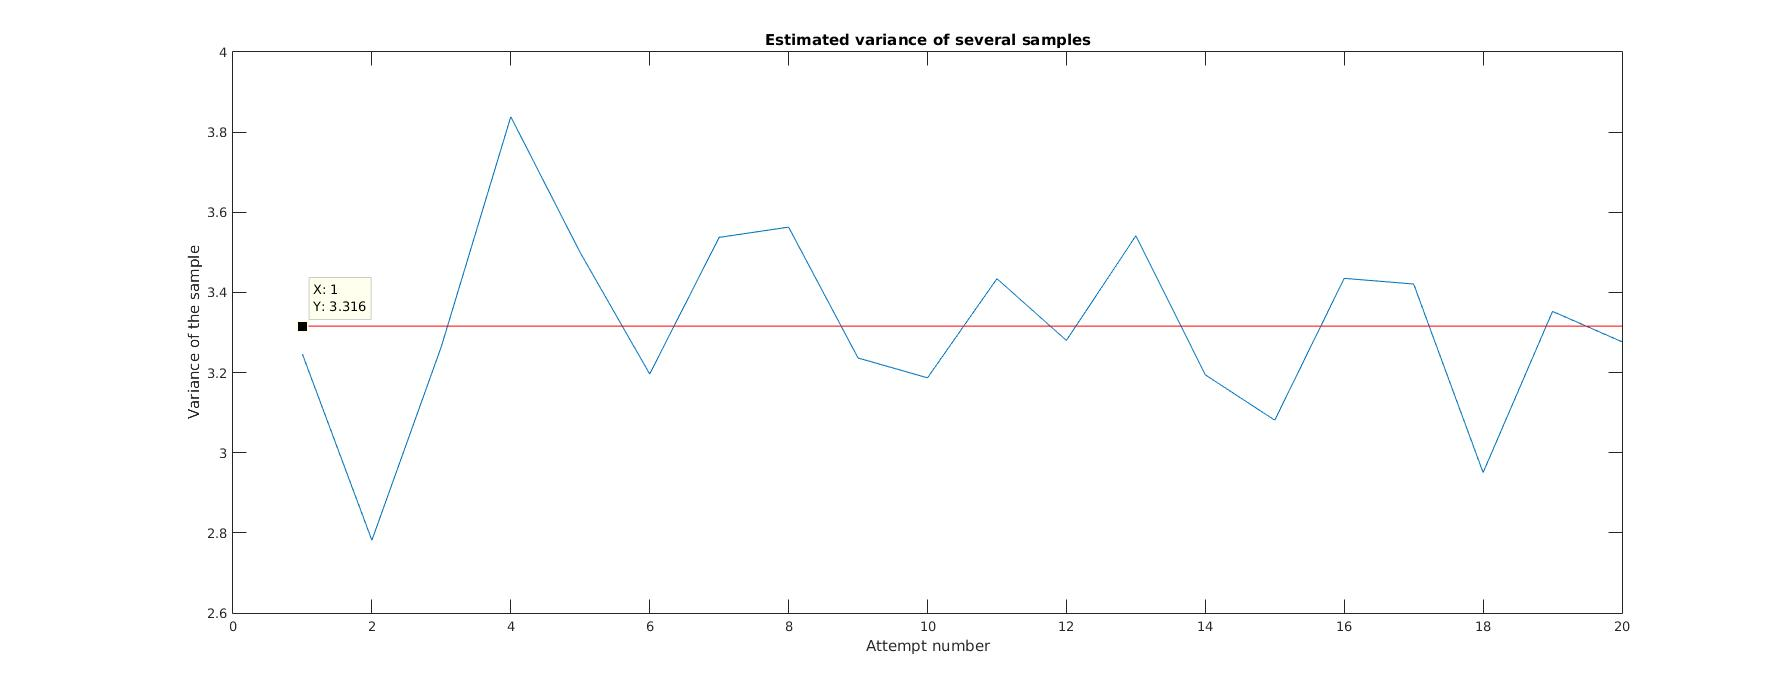
\includegraphics[scale = 0.37]{var_hmmrand}\label{hmmrand:var}}\\
    \subfloat[Mean of 10000 samples computed 20 times $E(E(X)) \simeq 0.7963$]{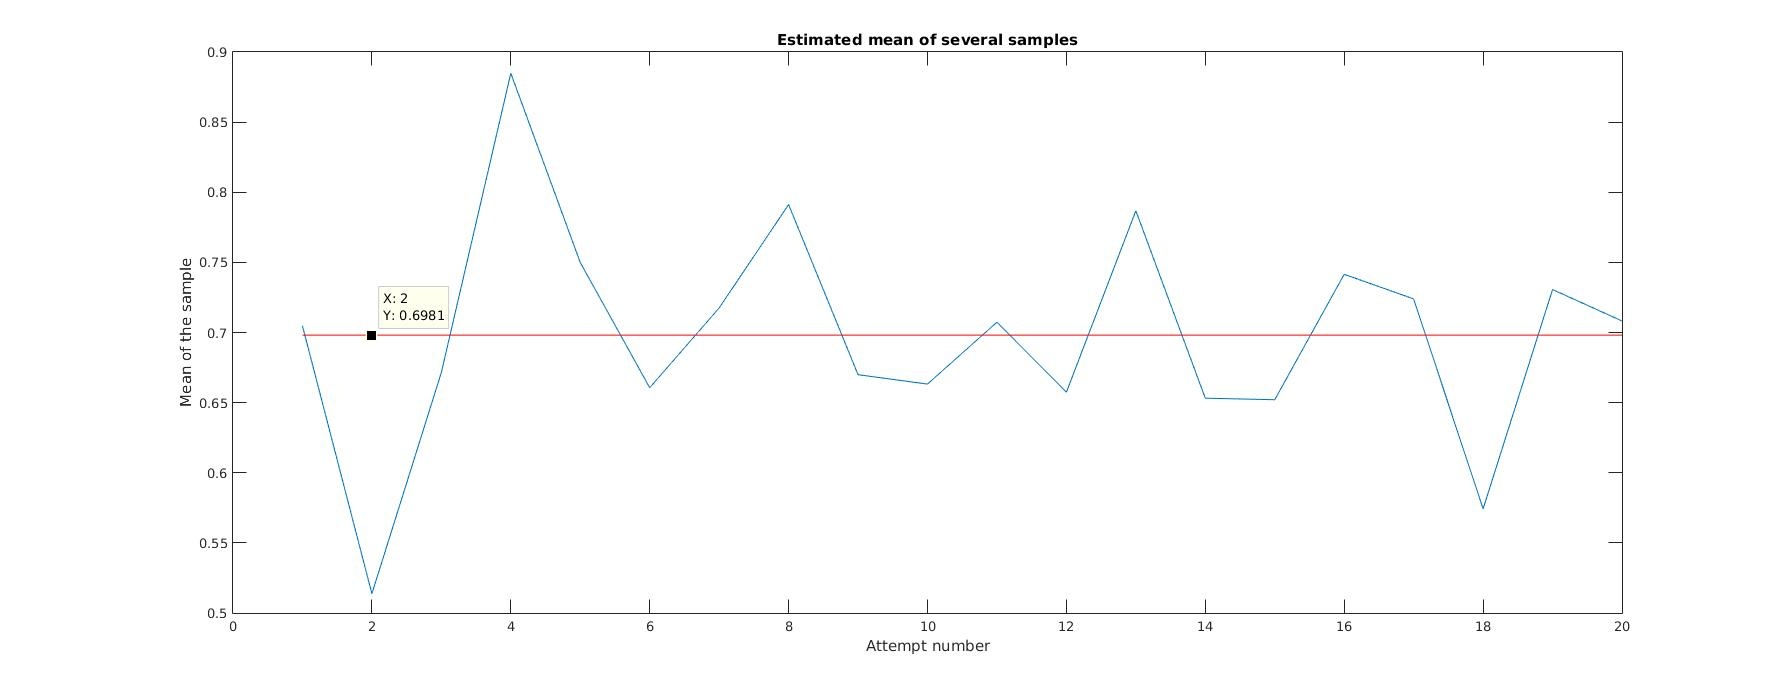
\includegraphics[scale = 0.37]{mean_hmmrand}\label{hmmrand:mean}}
\captionsetup{justification=centering}
    \caption{Validation of @HMM/rand\\\color{blue}{Blue : Plot of the 20 attempts}\\\color{red}{Red : Mean over the 20 attempts}}
\end{figure}
\pagebreak
\section{HMM behavior 1/2}
For this part, we changed the behavior of the @HMM/rand function, in order to get a vector from $b_{1}$ (not a scalar like the previous question). So here, each sample is a vector $x_{t} \sim N(\mu_j,\sigma_j^2)$ of size 500 (where j=1 or 2).

The following figure shows the 500 scalars from the process.

% \img{hmm_different_mean}{0.7}{Output data sample for two different means}

\img{etude_hmmrand}{0.4}{Plot of 500 contiguous $X_t$, the two states are defined as follow : $b_1(x) = N(0,1)$ and $b_2(x) = N(3,2)$}
\begin{pushright}{Observation}
After repeating the same code used to plot figure \ref{etude_hmmrand} several times, we confirmed the well behaving of the HMM. It is for likely to begin in state 1, and the system succeed in jumping into state 2, it will spend on this state than in state 1. When the means are different, it is pretty easy to find out the state sequence.
\end{pushright}
\pagebreak
\section{HMM behavior 2/2}
We now modify the mean of $b_{2}$, $\mu_{2}$ so that it is equal to $\mu_{1}$ : $\mu_{1}=\mu_{2}=0$.

We can easily notice a change with the previous HMM. On the figure below are represented a sample produced while the state was 1 in blue, and when the state was 2 in red :

\img{hmm_same_mean}{0.4}{Plot of 500 contiguous $X_t$, the two states are defined as follow : $b_1(x) = N(0,1)$ and $b_2(x) = N(0,2)$}
% 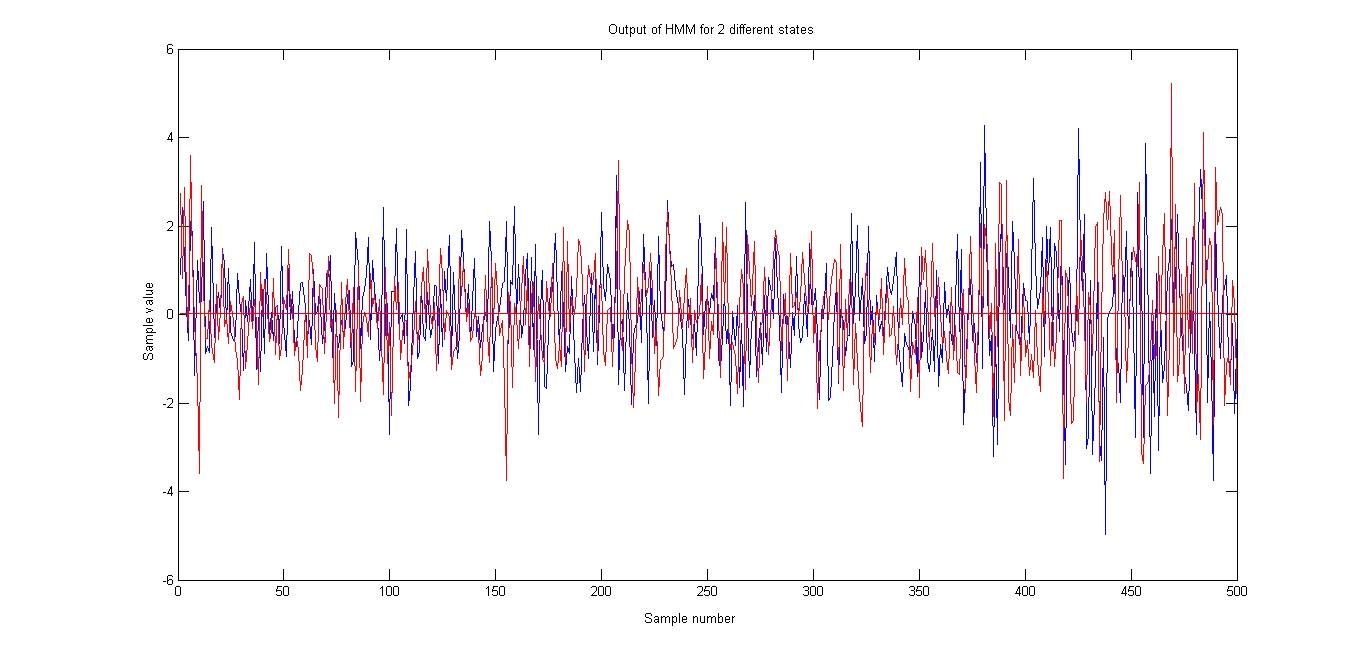
\includegraphics[width=15cm]{Question_5_mean_bis.jpg}
\begin{pushright}{Observation}
The sequence of state should be equivalent\footnote{ in term of probability of jumping from one state to another.} as the previous configuration. But only by considering the samples, when both means are equal, it is far more difficult to infer the state sequence. We can assume that the samples ``far'' from the mean are produced in state 2 (since the standard deviation is greater in state 2) but it is not a reliable assumption. 
\end{pushright}

\section{Finite-duration HMMs}
The implementation works with finite duration Markov chain.\\
We defined a transition matrix $A = \begin{pmatrix}
  0.6 & 0.3 & 0.1\\
  0.5 & 0.4 & 0.1\\
\end{pmatrix}$ for a Markov chain, then a HMM based on this Markov chain, and the call to @HMM/rand returns the correct information. The difference is that we don't know how long the sequence is since we don't know precisely when the system will jump in the exit state (state 3).
Here are three examples of several state sequences generated with three calls to @HMM/rand :\\
$S_1 =[ 1	2	2	1	1	2	1	2	2	1	1	2	1	1	1	1	1	2 3]$\\
$S_2 = [1	1	1	2	1	1	1	2	2	2	1	2	2	2	1	1	1	1	1	1	2	1	2	1	1	1	1	1	2	1	2	1	1	1	1	1	1	2	2	2	1	1	1	2	2	1	1 3]$\\
$S_3 = [1	2	1	2	1	1	2	2	1	2	2	1 3]$\\

\section{Output vectors}
The @HMM/rand function has been tested and works good when the Output Distributions returns both vectors and scalars.


\end{document}
